\documentclass[1p]{elsarticle_modified}
%\bibliographystyle{elsarticle-num}

%\usepackage[colorlinks]{hyperref}
%\usepackage{abbrmath_seonhwa} %\Abb, \Ascr, \Acal ,\Abf, \Afrak
\usepackage{amsfonts}
\usepackage{amssymb}
\usepackage{amsmath}
\usepackage{amsthm}
\usepackage{scalefnt}
\usepackage{amsbsy}
\usepackage{kotex}
\usepackage{caption}
\usepackage{subfig}
\usepackage{color}
\usepackage{graphicx}
\usepackage{xcolor} %% white, black, red, green, blue, cyan, magenta, yellow
\usepackage{float}
\usepackage{setspace}
\usepackage{hyperref}

\usepackage{tikz}
\usetikzlibrary{arrows}

\usepackage{multirow}
\usepackage{array} % fixed length table
\usepackage{hhline}

%%%%%%%%%%%%%%%%%%%%%
\makeatletter
\renewcommand*\env@matrix[1][\arraystretch]{%
	\edef\arraystretch{#1}%
	\hskip -\arraycolsep
	\let\@ifnextchar\new@ifnextchar
	\array{*\c@MaxMatrixCols c}}
\makeatother %https://tex.stackexchange.com/questions/14071/how-can-i-increase-the-line-spacing-in-a-matrix
%%%%%%%%%%%%%%%

\usepackage[normalem]{ulem}

\newcommand{\msout}[1]{\ifmmode\text{\sout{\ensuremath{#1}}}\else\sout{#1}\fi}
%SOURCE: \msout is \stkout macro in https://tex.stackexchange.com/questions/20609/strikeout-in-math-mode

\newcommand{\cancel}[1]{
	\ifmmode
	{\color{red}\msout{#1}}
	\else
	{\color{red}\sout{#1}}
	\fi
}

\newcommand{\add}[1]{
	{\color{blue}\uwave{#1}}
}

\newcommand{\replace}[2]{
	\ifmmode
	{\color{red}\msout{#1}}{\color{blue}\uwave{#2}}
	\else
	{\color{red}\sout{#1}}{\color{blue}\uwave{#2}}
	\fi
}

\newcommand{\Sol}{\mathcal{S}} %segment
\newcommand{\D}{D} %diagram
\newcommand{\A}{\mathcal{A}} %arc


%%%%%%%%%%%%%%%%%%%%%%%%%%%%%5 test

\def\sl{\operatorname{\textup{SL}}(2,\Cbb)}
\def\psl{\operatorname{\textup{PSL}}(2,\Cbb)}
\def\quan{\mkern 1mu \triangleright \mkern 1mu}

\theoremstyle{definition}
\newtheorem{thm}{Theorem}[section]
\newtheorem{prop}[thm]{Proposition}
\newtheorem{lem}[thm]{Lemma}
\newtheorem{ques}[thm]{Question}
\newtheorem{cor}[thm]{Corollary}
\newtheorem{defn}[thm]{Definition}
\newtheorem{exam}[thm]{Example}
\newtheorem{rmk}[thm]{Remark}
\newtheorem{alg}[thm]{Algorithm}

\newcommand{\I}{\sqrt{-1}}
\begin{document}

%\begin{frontmatter}
%
%\title{Boundary parabolic representations of knots up to 8 crossings}
%
%%% Group authors per affiliation:
%\author{Yunhi Cho} 
%\address{Department of Mathematics, University of Seoul, Seoul, Korea}
%\ead{yhcho@uos.ac.kr}
%
%
%\author{Seonhwa Kim} %\fnref{s_kim}}
%\address{Center for Geometry and Physics, Institute for Basic Science, Pohang, 37673, Korea}
%\ead{ryeona17@ibs.re.kr}
%
%\author{Hyuk Kim}
%\address{Department of Mathematical Sciences, Seoul National University, Seoul 08826, Korea}
%\ead{hyukkim@snu.ac.kr}
%
%\author{Seokbeom Yoon}
%\address{Department of Mathematical Sciences, Seoul National University, Seoul, 08826,  Korea}
%\ead{sbyoon15@snu.ac.kr}
%
%\begin{abstract}
%We find all boundary parabolic representation of knots up to 8 crossings.
%
%\end{abstract}
%\begin{keyword}
%    \MSC[2010] 57M25 
%\end{keyword}
%
%\end{frontmatter}

%\linenumbers
%\tableofcontents
%
\newcommand\colored[1]{\textcolor{white}{\rule[-0.35ex]{0.8em}{1.4ex}}\kern-0.8em\color{red} #1}%
%\newcommand\colored[1]{\textcolor{white}{ #1}\kern-2.17ex	\textcolor{white}{ #1}\kern-1.81ex	\textcolor{white}{ #1}\kern-2.15ex\color{red}#1	}

{\Large $\underline{12a_{0138}~(K12a_{0138})}$}

\setlength{\tabcolsep}{10pt}
\renewcommand{\arraystretch}{1.6}
\vspace{1cm}\begin{tabular}{m{100pt}>{\centering\arraybackslash}m{274pt}}
\multirow{5}{120pt}{
	\centering
	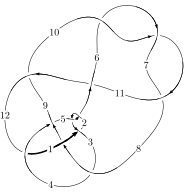
\includegraphics[width=112pt]{../../../GIT/diagram.site/Diagrams/png/939_12a_0138.png}\\
\ \ \ A knot diagram\footnotemark}&
\allowdisplaybreaks
\textbf{Linearized knot diagam} \\
\cline{2-2}
 &
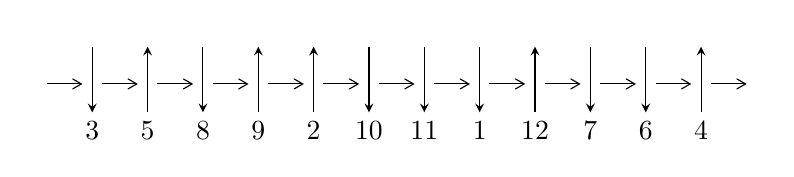
\begin{tikzpicture}[x=20pt, y=17pt]
	% nodes
	\node (C0) at (0, 0) {};
	\node (C1) at (1, 0) {};
	\node (C1U) at (1, +1) {};
	\node (C1D) at (1, -1) {3};

	\node (C2) at (2, 0) {};
	\node (C2U) at (2, +1) {};
	\node (C2D) at (2, -1) {5};

	\node (C3) at (3, 0) {};
	\node (C3U) at (3, +1) {};
	\node (C3D) at (3, -1) {8};

	\node (C4) at (4, 0) {};
	\node (C4U) at (4, +1) {};
	\node (C4D) at (4, -1) {9};

	\node (C5) at (5, 0) {};
	\node (C5U) at (5, +1) {};
	\node (C5D) at (5, -1) {2};

	\node (C6) at (6, 0) {};
	\node (C6U) at (6, +1) {};
	\node (C6D) at (6, -1) {10};

	\node (C7) at (7, 0) {};
	\node (C7U) at (7, +1) {};
	\node (C7D) at (7, -1) {11};

	\node (C8) at (8, 0) {};
	\node (C8U) at (8, +1) {};
	\node (C8D) at (8, -1) {1};

	\node (C9) at (9, 0) {};
	\node (C9U) at (9, +1) {};
	\node (C9D) at (9, -1) {12};

	\node (C10) at (10, 0) {};
	\node (C10U) at (10, +1) {};
	\node (C10D) at (10, -1) {7};

	\node (C11) at (11, 0) {};
	\node (C11U) at (11, +1) {};
	\node (C11D) at (11, -1) {6};

	\node (C12) at (12, 0) {};
	\node (C12U) at (12, +1) {};
	\node (C12D) at (12, -1) {4};
	\node (C13) at (13, 0) {};

	% arrows
	\draw[->,>={angle 60}]
	(C0) edge (C1) (C1) edge (C2) (C2) edge (C3) (C3) edge (C4) (C4) edge (C5) (C5) edge (C6) (C6) edge (C7) (C7) edge (C8) (C8) edge (C9) (C9) edge (C10) (C10) edge (C11) (C11) edge (C12) (C12) edge (C13) ;	\draw[->,>=stealth]
	(C1U) edge (C1D) (C2D) edge (C2U) (C3U) edge (C3D) (C4D) edge (C4U) (C5D) edge (C5U) (C6U) edge (C6D) (C7U) edge (C7D) (C8U) edge (C8D) (C9D) edge (C9U) (C10U) edge (C10D) (C11U) edge (C11D) (C12D) edge (C12U) ;
	\end{tikzpicture} \\
\hhline{~~} \\& 
\textbf{Solving Sequence} \\ \cline{2-2} 
 &
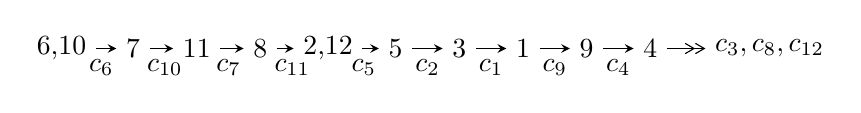
\begin{tikzpicture}[x=23pt, y=7pt]
	% node
	\node (A0) at (-1/8, 0) {6,10};
	\node (A1) at (1, 0) {7};
	\node (A2) at (2, 0) {11};
	\node (A3) at (3, 0) {8};
	\node (A4) at (65/16, 0) {2,12};
	\node (A5) at (41/8, 0) {5};
	\node (A6) at (49/8, 0) {3};
	\node (A7) at (57/8, 0) {1};
	\node (A8) at (65/8, 0) {9};
	\node (A9) at (73/8, 0) {4};
	\node (C1) at (1/2, -1) {$c_{6}$};
	\node (C2) at (3/2, -1) {$c_{10}$};
	\node (C3) at (5/2, -1) {$c_{7}$};
	\node (C4) at (7/2, -1) {$c_{11}$};
	\node (C5) at (37/8, -1) {$c_{5}$};
	\node (C6) at (45/8, -1) {$c_{2}$};
	\node (C7) at (53/8, -1) {$c_{1}$};
	\node (C8) at (61/8, -1) {$c_{9}$};
	\node (C9) at (69/8, -1) {$c_{4}$};
	\node (A10) at (11, 0) {$c_{3},c_{8},c_{12}$};

	% edge
	\draw[->,>=stealth]	
	(A0) edge (A1) (A1) edge (A2) (A2) edge (A3) (A3) edge (A4) (A4) edge (A5) (A5) edge (A6) (A6) edge (A7) (A7) edge (A8) (A8) edge (A9) ;
	\draw[->>,>={angle 60}]	
	(A9) edge (A10);
\end{tikzpicture} \\ 

\end{tabular} \\

\footnotetext{
The image of knot diagram is generated by the software ``\textbf{Draw programme}" developed by Andrew Bartholomew(\url{http://www.layer8.co.uk/maths/draw/index.htm\#Running-draw}), where we modified some parts for our purpose(\url{https://github.com/CATsTAILs/LinksPainter}).
}\phantom \\ \newline 
\centering \textbf{Ideals for irreducible components\footnotemark of $X_{\text{par}}$} 
 
\begin{align*}
I^u_{1}&=\langle 
7.19471\times10^{73} u^{112}-1.22414\times10^{74} u^{111}+\cdots+1.80916\times10^{73} b+6.97020\times10^{73},\\
\phantom{I^u_{1}}&\phantom{= \langle  }-1.81957\times10^{74} u^{112}+3.28712\times10^{74} u^{111}+\cdots+1.80916\times10^{73} a-1.87404\times10^{74},\\
\phantom{I^u_{1}}&\phantom{= \langle  }u^{113}-3 u^{112}+\cdots-2 u-1\rangle \\
I^u_{2}&=\langle 
b+a+1,\;a^2+3 a+3,\;u-1\rangle \\
\\
\end{align*}
\raggedright * 2 irreducible components of $\dim_{\mathbb{C}}=0$, with total 115 representations.\\
\footnotetext{All coefficients of polynomials are rational numbers. But the coefficients are sometimes approximated in decimal forms when there is not enough margin.}
\newpage
\renewcommand{\arraystretch}{1}
\centering \section*{I. $I^u_{1}= \langle 7.19\times10^{73} u^{112}-1.22\times10^{74} u^{111}+\cdots+1.81\times10^{73} b+6.97\times10^{73},\;-1.82\times10^{74} u^{112}+3.29\times10^{74} u^{111}+\cdots+1.81\times10^{73} a-1.87\times10^{74},\;u^{113}-3 u^{112}+\cdots-2 u-1 \rangle$}
\flushleft \textbf{(i) Arc colorings}\\
\begin{tabular}{m{7pt} m{180pt} m{7pt} m{180pt} }
\flushright $a_{6}=$&$\begin{pmatrix}1\\0\end{pmatrix}$ \\
\flushright $a_{10}=$&$\begin{pmatrix}0\\u\end{pmatrix}$ \\
\flushright $a_{7}=$&$\begin{pmatrix}1\\u^2\end{pmatrix}$ \\
\flushright $a_{11}=$&$\begin{pmatrix}- u\\- u^3+u\end{pmatrix}$ \\
\flushright $a_{8}=$&$\begin{pmatrix}- u^2+1\\- u^4+2 u^2\end{pmatrix}$ \\
\flushright $a_{2}=$&$\begin{pmatrix}10.0575 u^{112}-18.1693 u^{111}+\cdots+29.5396 u+10.3586\\-3.97683 u^{112}+6.76633 u^{111}+\cdots-13.0851 u-3.85273\end{pmatrix}$ \\
\flushright $a_{12}=$&$\begin{pmatrix}u^3-2 u\\- u^3+u\end{pmatrix}$ \\
\flushright $a_{5}=$&$\begin{pmatrix}21.7820 u^{112}-39.2061 u^{111}+\cdots+48.7260 u+19.4581\\-3.21144 u^{112}+5.39167 u^{111}+\cdots-11.0344 u-4.09903\end{pmatrix}$ \\
\flushright $a_{3}=$&$\begin{pmatrix}18.8353 u^{112}-34.2427 u^{111}+\cdots+38.5483 u+15.7723\\-3.75718 u^{112}+6.19544 u^{111}+\cdots-11.7379 u-4.57583\end{pmatrix}$ \\
\flushright $a_{1}=$&$\begin{pmatrix}-2.58530 u^{112}+4.46215 u^{111}+\cdots-2.91973 u-2.46253\\0.126934 u^{112}-0.107623 u^{111}+\cdots-0.558030 u-0.562200\end{pmatrix}$ \\
\flushright $a_{9}=$&$\begin{pmatrix}- u^7+4 u^5-4 u^3\\u^7-3 u^5+2 u^3+u\end{pmatrix}$ \\
\flushright $a_{4}=$&$\begin{pmatrix}15.1071 u^{112}-28.0166 u^{111}+\cdots+31.2262 u+13.6875\\6.59937 u^{112}-12.6329 u^{111}+\cdots+16.3813 u+4.92547\end{pmatrix}$\\&\end{tabular}
\flushleft \textbf{(ii) Obstruction class $= -1$}\\~\\
\flushleft \textbf{(iii) Cusp Shapes $= -21.9603 u^{112}+39.6262 u^{111}+\cdots-14.3575 u-5.90643$}\\~\\
\newpage\renewcommand{\arraystretch}{1}
\flushleft \textbf{(iv) u-Polynomials at the component}\newline \\
\begin{tabular}{m{50pt}|m{274pt}}
Crossings & \hspace{64pt}u-Polynomials at each crossing \\
\hline $$\begin{aligned}c_{1}\end{aligned}$$&$\begin{aligned}
&u^{113}+48 u^{112}+\cdots+55 u-1
\end{aligned}$\\
\hline $$\begin{aligned}c_{2},c_{5}\end{aligned}$$&$\begin{aligned}
&u^{113}+2 u^{112}+\cdots-5 u-1
\end{aligned}$\\
\hline $$\begin{aligned}c_{3}\end{aligned}$$&$\begin{aligned}
&u^{113}+60 u^{111}+\cdots-47 u+1
\end{aligned}$\\
\hline $$\begin{aligned}c_{4}\end{aligned}$$&$\begin{aligned}
&u^{113}+2 u^{112}+\cdots+1009 u+347
\end{aligned}$\\
\hline $$\begin{aligned}c_{6},c_{7},c_{10}\end{aligned}$$&$\begin{aligned}
&u^{113}+3 u^{112}+\cdots-2 u+1
\end{aligned}$\\
\hline $$\begin{aligned}c_{8}\end{aligned}$$&$\begin{aligned}
&u^{113}+7 u^{112}+\cdots+u^2+1
\end{aligned}$\\
\hline $$\begin{aligned}c_{9}\end{aligned}$$&$\begin{aligned}
&u^{113}+23 u^{112}+\cdots+6255814 u+309047
\end{aligned}$\\
\hline $$\begin{aligned}c_{11}\end{aligned}$$&$\begin{aligned}
&u^{113}-3 u^{112}+\cdots+1280 u-1088
\end{aligned}$\\
\hline $$\begin{aligned}c_{12}\end{aligned}$$&$\begin{aligned}
&u^{113}+11 u^{112}+\cdots+12 u+4
\end{aligned}$\\
\hline
\end{tabular}\\~\\
\newpage\renewcommand{\arraystretch}{1}
\flushleft \textbf{(v) Riley Polynomials at the component}\newline \\
\begin{tabular}{m{50pt}|m{274pt}}
Crossings & \hspace{64pt}Riley Polynomials at each crossing \\
\hline $$\begin{aligned}c_{1}\end{aligned}$$&$\begin{aligned}
&y^{113}+36 y^{112}+\cdots+3831 y-1
\end{aligned}$\\
\hline $$\begin{aligned}c_{2},c_{5}\end{aligned}$$&$\begin{aligned}
&y^{113}+48 y^{112}+\cdots+55 y-1
\end{aligned}$\\
\hline $$\begin{aligned}c_{3}\end{aligned}$$&$\begin{aligned}
&y^{113}+120 y^{112}+\cdots+463 y-1
\end{aligned}$\\
\hline $$\begin{aligned}c_{4}\end{aligned}$$&$\begin{aligned}
&y^{113}+128 y^{112}+\cdots-8247513 y-120409
\end{aligned}$\\
\hline $$\begin{aligned}c_{6},c_{7},c_{10}\end{aligned}$$&$\begin{aligned}
&y^{113}-103 y^{112}+\cdots-2 y-1
\end{aligned}$\\
\hline $$\begin{aligned}c_{8}\end{aligned}$$&$\begin{aligned}
&y^{113}+9 y^{112}+\cdots-2 y-1
\end{aligned}$\\
\hline $$\begin{aligned}c_{9}\end{aligned}$$&$\begin{aligned}
&y^{113}+53 y^{112}+\cdots-1833344062454 y-95510048209
\end{aligned}$\\
\hline $$\begin{aligned}c_{11}\end{aligned}$$&$\begin{aligned}
&y^{113}-17 y^{112}+\cdots+72743552 y-1183744
\end{aligned}$\\
\hline $$\begin{aligned}c_{12}\end{aligned}$$&$\begin{aligned}
&y^{113}+15 y^{112}+\cdots-280 y-16
\end{aligned}$\\
\hline
\end{tabular}\\~\\
\newpage\flushleft \textbf{(vi) Complex Volumes and Cusp Shapes}
$$\begin{array}{c|c|c}  
\text{Solutions to }I^u_{1}& \I (\text{vol} + \sqrt{-1}CS) & \text{Cusp shape}\\
 \hline 
\begin{aligned}
u &= \phantom{-}0.939909 + 0.317543 I \\
a &= \phantom{-}1.46055 - 0.18139 I \\
b &= -0.368917 + 0.830267 I\end{aligned}
 & -2.13808 - 1.37165 I & \phantom{-0.000000 } 0 \\ \hline\begin{aligned}
u &= \phantom{-}0.939909 - 0.317543 I \\
a &= \phantom{-}1.46055 + 0.18139 I \\
b &= -0.368917 - 0.830267 I\end{aligned}
 & -2.13808 + 1.37165 I & \phantom{-0.000000 } 0 \\ \hline\begin{aligned}
u &= \phantom{-}0.752167 + 0.473634 I \\
a &= \phantom{-}0.826598 + 0.274339 I \\
b &= -0.455174 - 0.969053 I\end{aligned}
 & -2.81213 + 1.98997 I & \phantom{-0.000000 } 0 \\ \hline\begin{aligned}
u &= \phantom{-}0.752167 - 0.473634 I \\
a &= \phantom{-}0.826598 - 0.274339 I \\
b &= -0.455174 + 0.969053 I\end{aligned}
 & -2.81213 - 1.98997 I & \phantom{-0.000000 } 0 \\ \hline\begin{aligned}
u &= -1.118790 + 0.027576 I \\
a &= -0.980417 - 0.453269 I \\
b &= \phantom{-}0.925019 + 0.474762 I\end{aligned}
 & \phantom{-}0.74089 + 1.69233 I & \phantom{-0.000000 } 0 \\ \hline\begin{aligned}
u &= -1.118790 - 0.027576 I \\
a &= -0.980417 + 0.453269 I \\
b &= \phantom{-}0.925019 - 0.474762 I\end{aligned}
 & \phantom{-}0.74089 - 1.69233 I & \phantom{-0.000000 } 0 \\ \hline\begin{aligned}
u &= \phantom{-}0.579977 + 0.611709 I \\
a &= \phantom{-}1.344920 + 0.261692 I \\
b &= -0.423750 + 0.967531 I\end{aligned}
 & -2.99500 - 3.68548 I & \phantom{-0.000000 } 0 \\ \hline\begin{aligned}
u &= \phantom{-}0.579977 - 0.611709 I \\
a &= \phantom{-}1.344920 - 0.261692 I \\
b &= -0.423750 - 0.967531 I\end{aligned}
 & -2.99500 + 3.68548 I & \phantom{-0.000000 } 0 \\ \hline\begin{aligned}
u &= \phantom{-}1.15862\phantom{ +0.000000I} \\
a &= \phantom{-}0.574458\phantom{ +0.000000I} \\
b &= \phantom{-}0.129833\phantom{ +0.000000I}\end{aligned}
 & -1.97009\phantom{ +0.000000I} & \phantom{-0.000000 } 0 \\ \hline\begin{aligned}
u &= \phantom{-}0.323055 + 0.768075 I \\
a &= \phantom{-}2.28499 - 0.15615 I \\
b &= -0.514948 + 0.996717 I\end{aligned}
 & -1.39021 - 6.40201 I & \phantom{-0.000000 } 0\\
 \hline 
 \end{array}$$\newpage$$\begin{array}{c|c|c}  
\text{Solutions to }I^u_{1}& \I (\text{vol} + \sqrt{-1}CS) & \text{Cusp shape}\\
 \hline 
\begin{aligned}
u &= \phantom{-}0.323055 - 0.768075 I \\
a &= \phantom{-}2.28499 + 0.15615 I \\
b &= -0.514948 - 0.996717 I\end{aligned}
 & -1.39021 + 6.40201 I & \phantom{-0.000000 } 0 \\ \hline\begin{aligned}
u &= -1.167310 + 0.082409 I \\
a &= -1.61291 - 0.08377 I \\
b &= \phantom{-}0.732275 + 1.080280 I\end{aligned}
 & -1.03203 + 4.35287 I & \phantom{-0.000000 } 0 \\ \hline\begin{aligned}
u &= -1.167310 - 0.082409 I \\
a &= -1.61291 + 0.08377 I \\
b &= \phantom{-}0.732275 - 1.080280 I\end{aligned}
 & -1.03203 - 4.35287 I & \phantom{-0.000000 } 0 \\ \hline\begin{aligned}
u &= \phantom{-}0.440456 + 0.694712 I \\
a &= \phantom{-}0.138212 + 0.304488 I \\
b &= -0.351572 - 0.923192 I\end{aligned}
 & -2.54432 - 0.78650 I & \phantom{-0.000000 } 0 \\ \hline\begin{aligned}
u &= \phantom{-}0.440456 - 0.694712 I \\
a &= \phantom{-}0.138212 - 0.304488 I \\
b &= -0.351572 + 0.923192 I\end{aligned}
 & -2.54432 + 0.78650 I & \phantom{-0.000000 } 0 \\ \hline\begin{aligned}
u &= -1.150760 + 0.263291 I \\
a &= \phantom{-}0.884861 - 0.795944 I \\
b &= -0.806370 + 0.549939 I\end{aligned}
 & \phantom{-}1.48117 + 5.52965 I & \phantom{-0.000000 } 0 \\ \hline\begin{aligned}
u &= -1.150760 - 0.263291 I \\
a &= \phantom{-}0.884861 + 0.795944 I \\
b &= -0.806370 - 0.549939 I\end{aligned}
 & \phantom{-}1.48117 - 5.52965 I & \phantom{-0.000000 } 0 \\ \hline\begin{aligned}
u &= -0.649038 + 0.499158 I \\
a &= \phantom{-}0.799156 - 0.174595 I \\
b &= -0.645108 + 1.123390 I\end{aligned}
 & -1.72359 - 10.60720 I & \phantom{-0.000000 } 0 \\ \hline\begin{aligned}
u &= -0.649038 - 0.499158 I \\
a &= \phantom{-}0.799156 + 0.174595 I \\
b &= -0.645108 - 1.123390 I\end{aligned}
 & -1.72359 + 10.60720 I & \phantom{-0.000000 } 0 \\ \hline\begin{aligned}
u &= -0.341872 + 0.735602 I \\
a &= \phantom{-}2.63336 - 0.13250 I \\
b &= -0.663628 - 1.137570 I\end{aligned}
 & -0.6241 + 14.8733 I & \phantom{-0.000000 } 0. - 10.48364 I\\
 \hline 
 \end{array}$$\newpage$$\begin{array}{c|c|c}  
\text{Solutions to }I^u_{1}& \I (\text{vol} + \sqrt{-1}CS) & \text{Cusp shape}\\
 \hline 
\begin{aligned}
u &= -0.341872 - 0.735602 I \\
a &= \phantom{-}2.63336 + 0.13250 I \\
b &= -0.663628 + 1.137570 I\end{aligned}
 & -0.6241 - 14.8733 I & \phantom{-0.000000 -}0. + 10.48364 I \\ \hline\begin{aligned}
u &= \phantom{-}1.191890 + 0.019067 I \\
a &= -4.44997 + 2.27032 I \\
b &= \phantom{-}0.534866 - 0.855939 I\end{aligned}
 & -2.14131 - 2.15135 I & \phantom{-0.000000 } 0 \\ \hline\begin{aligned}
u &= \phantom{-}1.191890 - 0.019067 I \\
a &= -4.44997 - 2.27032 I \\
b &= \phantom{-}0.534866 + 0.855939 I\end{aligned}
 & -2.14131 + 2.15135 I & \phantom{-0.000000 } 0 \\ \hline\begin{aligned}
u &= -0.325971 + 0.717414 I \\
a &= \phantom{-}1.00912 - 1.43916 I \\
b &= -0.916275 + 0.452303 I\end{aligned}
 & \phantom{-}1.46474 + 9.07915 I & \phantom{-0.000000 } 0. - 7.02875 I \\ \hline\begin{aligned}
u &= -0.325971 - 0.717414 I \\
a &= \phantom{-}1.00912 + 1.43916 I \\
b &= -0.916275 - 0.452303 I\end{aligned}
 & \phantom{-}1.46474 - 9.07915 I & \phantom{-0.000000 -}0. + 7.02875 I \\ \hline\begin{aligned}
u &= -1.182760 + 0.306456 I \\
a &= \phantom{-}1.92843 - 0.18354 I \\
b &= -0.652135 - 1.054830 I\end{aligned}
 & -0.04028 + 10.99740 I & \phantom{-0.000000 } 0 \\ \hline\begin{aligned}
u &= -1.182760 - 0.306456 I \\
a &= \phantom{-}1.92843 + 0.18354 I \\
b &= -0.652135 + 1.054830 I\end{aligned}
 & -0.04028 - 10.99740 I & \phantom{-0.000000 } 0 \\ \hline\begin{aligned}
u &= -0.627370 + 0.450096 I \\
a &= \phantom{-}1.102860 - 0.068589 I \\
b &= -0.866470 - 0.442386 I\end{aligned}
 & \phantom{-}0.32647 - 5.01240 I & -2.00000 + 1.72974 I \\ \hline\begin{aligned}
u &= -0.627370 - 0.450096 I \\
a &= \phantom{-}1.102860 + 0.068589 I \\
b &= -0.866470 + 0.442386 I\end{aligned}
 & \phantom{-}0.32647 + 5.01240 I & -2.00000 - 1.72974 I \\ \hline\begin{aligned}
u &= -0.011515 + 0.764522 I \\
a &= \phantom{-}1.78598 - 1.34153 I \\
b &= -0.631765 + 1.016450 I\end{aligned}
 & \phantom{-}3.55207 - 7.10523 I & \phantom{-}1.72920 + 7.58809 I\\
 \hline 
 \end{array}$$\newpage$$\begin{array}{c|c|c}  
\text{Solutions to }I^u_{1}& \I (\text{vol} + \sqrt{-1}CS) & \text{Cusp shape}\\
 \hline 
\begin{aligned}
u &= -0.011515 - 0.764522 I \\
a &= \phantom{-}1.78598 + 1.34153 I \\
b &= -0.631765 - 1.016450 I\end{aligned}
 & \phantom{-}3.55207 + 7.10523 I & \phantom{-}1.72920 - 7.58809 I \\ \hline\begin{aligned}
u &= -0.357793 + 0.666831 I \\
a &= -1.078110 - 0.253263 I \\
b &= -0.030920 + 1.288310 I\end{aligned}
 & -4.91041 + 6.36723 I & -6.53571 - 8.04968 I \\ \hline\begin{aligned}
u &= -0.357793 - 0.666831 I \\
a &= -1.078110 + 0.253263 I \\
b &= -0.030920 - 1.288310 I\end{aligned}
 & -4.91041 - 6.36723 I & -6.53571 + 8.04968 I \\ \hline\begin{aligned}
u &= \phantom{-}1.208510 + 0.330567 I \\
a &= \phantom{-}0.440418 + 0.637304 I \\
b &= -0.601288 - 0.975849 I\end{aligned}
 & -0.20340 + 3.14702 I & \phantom{-0.000000 } 0 \\ \hline\begin{aligned}
u &= \phantom{-}1.208510 - 0.330567 I \\
a &= \phantom{-}0.440418 - 0.637304 I \\
b &= -0.601288 + 0.975849 I\end{aligned}
 & -0.20340 - 3.14702 I & \phantom{-0.000000 } 0 \\ \hline\begin{aligned}
u &= \phantom{-}0.255939 + 0.693140 I \\
a &= \phantom{-}0.783379 + 1.097760 I \\
b &= -0.343556 - 0.527140 I\end{aligned}
 & -0.04039 - 2.38375 I & -1.98371 + 5.90852 I \\ \hline\begin{aligned}
u &= \phantom{-}0.255939 - 0.693140 I \\
a &= \phantom{-}0.783379 - 1.097760 I \\
b &= -0.343556 + 0.527140 I\end{aligned}
 & -0.04039 + 2.38375 I & -1.98371 - 5.90852 I \\ \hline\begin{aligned}
u &= -0.051929 + 0.725337 I \\
a &= \phantom{-}2.13698 + 0.72891 I \\
b &= -0.735643 - 0.596633 I\end{aligned}
 & \phantom{-}4.81430 - 1.88544 I & \phantom{-}4.72473 + 1.60361 I \\ \hline\begin{aligned}
u &= -0.051929 - 0.725337 I \\
a &= \phantom{-}2.13698 - 0.72891 I \\
b &= -0.735643 + 0.596633 I\end{aligned}
 & \phantom{-}4.81430 + 1.88544 I & \phantom{-}4.72473 - 1.60361 I \\ \hline\begin{aligned}
u &= -1.269840 + 0.138595 I \\
a &= -0.220884 + 0.428106 I \\
b &= \phantom{-}0.189644 + 1.136810 I\end{aligned}
 & -4.83804 + 4.63939 I & \phantom{-0.000000 } 0\\
 \hline 
 \end{array}$$\newpage$$\begin{array}{c|c|c}  
\text{Solutions to }I^u_{1}& \I (\text{vol} + \sqrt{-1}CS) & \text{Cusp shape}\\
 \hline 
\begin{aligned}
u &= -1.269840 - 0.138595 I \\
a &= -0.220884 - 0.428106 I \\
b &= \phantom{-}0.189644 - 1.136810 I\end{aligned}
 & -4.83804 - 4.63939 I & \phantom{-0.000000 } 0 \\ \hline\begin{aligned}
u &= -0.514108 + 0.503712 I \\
a &= \phantom{-}1.036330 - 0.361962 I \\
b &= -0.073302 - 1.239800 I\end{aligned}
 & -5.57728 - 2.46347 I & -8.69302 + 1.29328 I \\ \hline\begin{aligned}
u &= -0.514108 - 0.503712 I \\
a &= \phantom{-}1.036330 + 0.361962 I \\
b &= -0.073302 + 1.239800 I\end{aligned}
 & -5.57728 + 2.46347 I & -8.69302 - 1.29328 I \\ \hline\begin{aligned}
u &= \phantom{-}1.257620 + 0.290271 I \\
a &= \phantom{-}1.63911 + 0.39912 I \\
b &= -0.669510 + 0.656393 I\end{aligned}
 & \phantom{-}0.76639 - 1.79202 I & \phantom{-0.000000 } 0 \\ \hline\begin{aligned}
u &= \phantom{-}1.257620 - 0.290271 I \\
a &= \phantom{-}1.63911 - 0.39912 I \\
b &= -0.669510 - 0.656393 I\end{aligned}
 & \phantom{-}0.76639 + 1.79202 I & \phantom{-0.000000 } 0 \\ \hline\begin{aligned}
u &= -0.300733 + 0.634297 I \\
a &= -2.69044 + 0.24594 I \\
b &= \phantom{-}0.652286 + 1.200950 I\end{aligned}
 & \phantom{-}0.19992 + 6.60671 I & \phantom{-}0.07217 - 12.10916 I \\ \hline\begin{aligned}
u &= -0.300733 - 0.634297 I \\
a &= -2.69044 - 0.24594 I \\
b &= \phantom{-}0.652286 - 1.200950 I\end{aligned}
 & \phantom{-}0.19992 - 6.60671 I & \phantom{-}0.07217 + 12.10916 I \\ \hline\begin{aligned}
u &= \phantom{-}1.297840 + 0.027388 I \\
a &= \phantom{-}1.04790 - 1.63196 I \\
b &= \phantom{-}0.286338 - 0.747497 I\end{aligned}
 & -3.22613 - 1.48459 I & \phantom{-0.000000 } 0 \\ \hline\begin{aligned}
u &= \phantom{-}1.297840 - 0.027388 I \\
a &= \phantom{-}1.04790 + 1.63196 I \\
b &= \phantom{-}0.286338 + 0.747497 I\end{aligned}
 & -3.22613 + 1.48459 I & \phantom{-0.000000 } 0 \\ \hline\begin{aligned}
u &= \phantom{-}0.234136 + 0.628805 I \\
a &= \phantom{-}0.318271 + 0.979558 I \\
b &= \phantom{-}0.027002 - 0.471357 I\end{aligned}
 & -0.07346 - 2.33823 I & -3.38006 + 5.78977 I\\
 \hline 
 \end{array}$$\newpage$$\begin{array}{c|c|c}  
\text{Solutions to }I^u_{1}& \I (\text{vol} + \sqrt{-1}CS) & \text{Cusp shape}\\
 \hline 
\begin{aligned}
u &= \phantom{-}0.234136 - 0.628805 I \\
a &= \phantom{-}0.318271 - 0.979558 I \\
b &= \phantom{-}0.027002 + 0.471357 I\end{aligned}
 & -0.07346 + 2.33823 I & -3.38006 - 5.78977 I \\ \hline\begin{aligned}
u &= -0.253157 + 0.618984 I \\
a &= -2.34577 + 0.07324 I \\
b &= \phantom{-}0.933553 + 0.670622 I\end{aligned}
 & \phantom{-}2.57361 + 4.20982 I & \phantom{-}6.47955 - 9.14983 I \\ \hline\begin{aligned}
u &= -0.253157 - 0.618984 I \\
a &= -2.34577 - 0.07324 I \\
b &= \phantom{-}0.933553 - 0.670622 I\end{aligned}
 & \phantom{-}2.57361 - 4.20982 I & \phantom{-}6.47955 + 9.14983 I \\ \hline\begin{aligned}
u &= \phantom{-}0.310571 + 0.587049 I \\
a &= -4.65059 - 1.98552 I \\
b &= \phantom{-}0.509350 - 0.916675 I\end{aligned}
 & -0.38515 - 3.92427 I & \phantom{-}1.8807 - 17.6364 I \\ \hline\begin{aligned}
u &= \phantom{-}0.310571 - 0.587049 I \\
a &= -4.65059 + 1.98552 I \\
b &= \phantom{-}0.509350 + 0.916675 I\end{aligned}
 & -0.38515 + 3.92427 I & \phantom{-}1.8807 + 17.6364 I \\ \hline\begin{aligned}
u &= -0.215249 + 0.601538 I \\
a &= -1.05368 + 1.43755 I \\
b &= \phantom{-}0.901782 - 0.257745 I\end{aligned}
 & \phantom{-}2.97908 + 0.86642 I & \phantom{-}8.54734 - 2.47415 I \\ \hline\begin{aligned}
u &= -0.215249 - 0.601538 I \\
a &= -1.05368 - 1.43755 I \\
b &= \phantom{-}0.901782 + 0.257745 I\end{aligned}
 & \phantom{-}2.97908 - 0.86642 I & \phantom{-}8.54734 + 2.47415 I \\ \hline\begin{aligned}
u &= \phantom{-}0.258441 + 0.568603 I \\
a &= -0.24006 - 3.99969 I \\
b &= \phantom{-}0.492878 + 0.781115 I\end{aligned}
 & \phantom{-}0.063611 + 0.181588 I & -10.94547 - 7.12456 I \\ \hline\begin{aligned}
u &= \phantom{-}0.258441 - 0.568603 I \\
a &= -0.24006 + 3.99969 I \\
b &= \phantom{-}0.492878 - 0.781115 I\end{aligned}
 & \phantom{-}0.063611 - 0.181588 I & -10.94547 + 7.12456 I \\ \hline\begin{aligned}
u &= \phantom{-}0.449623 + 0.413218 I \\
a &= \phantom{-}0.972889 - 0.131299 I \\
b &= -0.283957 + 0.017994 I\end{aligned}
 & -1.09683 - 0.93427 I & -5.40273 + 3.78636 I\\
 \hline 
 \end{array}$$\newpage$$\begin{array}{c|c|c}  
\text{Solutions to }I^u_{1}& \I (\text{vol} + \sqrt{-1}CS) & \text{Cusp shape}\\
 \hline 
\begin{aligned}
u &= \phantom{-}0.449623 - 0.413218 I \\
a &= \phantom{-}0.972889 + 0.131299 I \\
b &= -0.283957 - 0.017994 I\end{aligned}
 & -1.09683 + 0.93427 I & -5.40273 - 3.78636 I \\ \hline\begin{aligned}
u &= \phantom{-}0.342240 + 0.503546 I \\
a &= -0.76992 + 2.58082 I \\
b &= \phantom{-}0.455400 + 0.907374 I\end{aligned}
 & -0.692652 + 0.747510 I & \phantom{-}11.9814 + 9.3471 I \\ \hline\begin{aligned}
u &= \phantom{-}0.342240 - 0.503546 I \\
a &= -0.76992 - 2.58082 I \\
b &= \phantom{-}0.455400 - 0.907374 I\end{aligned}
 & -0.692652 - 0.747510 I & \phantom{-}11.9814 - 9.3471 I \\ \hline\begin{aligned}
u &= \phantom{-}1.388180 + 0.206751 I \\
a &= \phantom{-}0.197810 - 0.570262 I \\
b &= \phantom{-}0.878563 + 0.906512 I\end{aligned}
 & -3.29106 - 0.71548 I & \phantom{-0.000000 } 0 \\ \hline\begin{aligned}
u &= \phantom{-}1.388180 - 0.206751 I \\
a &= \phantom{-}0.197810 + 0.570262 I \\
b &= \phantom{-}0.878563 - 0.906512 I\end{aligned}
 & -3.29106 + 0.71548 I & \phantom{-0.000000 } 0 \\ \hline\begin{aligned}
u &= \phantom{-}1.389330 + 0.229302 I \\
a &= \phantom{-}0.032086 - 1.016630 I \\
b &= \phantom{-}0.985524 + 0.169001 I\end{aligned}
 & -2.15273 - 3.89237 I & \phantom{-0.000000 } 0 \\ \hline\begin{aligned}
u &= \phantom{-}1.389330 - 0.229302 I \\
a &= \phantom{-}0.032086 + 1.016630 I \\
b &= \phantom{-}0.985524 - 0.169001 I\end{aligned}
 & -2.15273 + 3.89237 I & \phantom{-0.000000 } 0 \\ \hline\begin{aligned}
u &= -1.395280 + 0.228734 I \\
a &= \phantom{-}0.022173 - 0.456532 I \\
b &= \phantom{-}0.318153 + 0.529929 I\end{aligned}
 & -5.25575 + 5.40772 I & \phantom{-0.000000 } 0 \\ \hline\begin{aligned}
u &= -1.395280 - 0.228734 I \\
a &= \phantom{-}0.022173 + 0.456532 I \\
b &= \phantom{-}0.318153 - 0.529929 I\end{aligned}
 & -5.25575 - 5.40772 I & \phantom{-0.000000 } 0 \\ \hline\begin{aligned}
u &= -1.40251 + 0.22262 I \\
a &= \phantom{-}0.20905 + 2.11697 I \\
b &= \phantom{-}0.515171 - 0.727283 I\end{aligned}
 & -5.25799 + 2.73945 I & \phantom{-0.000000 } 0\\
 \hline 
 \end{array}$$\newpage$$\begin{array}{c|c|c}  
\text{Solutions to }I^u_{1}& \I (\text{vol} + \sqrt{-1}CS) & \text{Cusp shape}\\
 \hline 
\begin{aligned}
u &= -1.40251 - 0.22262 I \\
a &= \phantom{-}0.20905 - 2.11697 I \\
b &= \phantom{-}0.515171 + 0.727283 I\end{aligned}
 & -5.25799 - 2.73945 I & \phantom{-0.000000 } 0 \\ \hline\begin{aligned}
u &= \phantom{-}1.40136 + 0.23957 I \\
a &= -1.22459 - 0.93674 I \\
b &= \phantom{-}0.982381 - 0.722917 I\end{aligned}
 & -2.71907 - 7.34999 I & \phantom{-0.000000 } 0 \\ \hline\begin{aligned}
u &= \phantom{-}1.40136 - 0.23957 I \\
a &= -1.22459 + 0.93674 I \\
b &= \phantom{-}0.982381 + 0.722917 I\end{aligned}
 & -2.71907 + 7.34999 I & \phantom{-0.000000 } 0 \\ \hline\begin{aligned}
u &= \phantom{-}1.41292 + 0.18059 I \\
a &= \phantom{-}0.524545 + 1.034890 I \\
b &= \phantom{-}0.524820 + 1.235330 I\end{aligned}
 & -6.26506 + 1.08823 I & \phantom{-0.000000 } 0 \\ \hline\begin{aligned}
u &= \phantom{-}1.41292 - 0.18059 I \\
a &= \phantom{-}0.524545 - 1.034890 I \\
b &= \phantom{-}0.524820 - 1.235330 I\end{aligned}
 & -6.26506 - 1.08823 I & \phantom{-0.000000 } 0 \\ \hline\begin{aligned}
u &= -0.170323 + 0.538397 I \\
a &= -0.88005 + 2.08855 I \\
b &= \phantom{-}0.766888 - 0.937064 I\end{aligned}
 & \phantom{-}1.75629 - 1.99035 I & \phantom{-}5.16557 + 2.88568 I \\ \hline\begin{aligned}
u &= -0.170323 - 0.538397 I \\
a &= -0.88005 - 2.08855 I \\
b &= \phantom{-}0.766888 + 0.937064 I\end{aligned}
 & \phantom{-}1.75629 + 1.99035 I & \phantom{-}5.16557 - 2.88568 I \\ \hline\begin{aligned}
u &= -1.42218 + 0.20369 I \\
a &= -0.34383 - 2.55067 I \\
b &= \phantom{-}0.444068 - 0.949016 I\end{aligned}
 & -6.33252 + 1.92115 I & \phantom{-0.000000 } 0 \\ \hline\begin{aligned}
u &= -1.42218 - 0.20369 I \\
a &= -0.34383 + 2.55067 I \\
b &= \phantom{-}0.444068 + 0.949016 I\end{aligned}
 & -6.33252 - 1.92115 I & \phantom{-0.000000 } 0 \\ \hline\begin{aligned}
u &= -1.42009 + 0.23097 I \\
a &= -3.25951 + 2.43167 I \\
b &= \phantom{-}0.517759 + 0.941725 I\end{aligned}
 & -5.93096 + 6.95191 I & \phantom{-0.000000 } 0\\
 \hline 
 \end{array}$$\newpage$$\begin{array}{c|c|c}  
\text{Solutions to }I^u_{1}& \I (\text{vol} + \sqrt{-1}CS) & \text{Cusp shape}\\
 \hline 
\begin{aligned}
u &= -1.42009 - 0.23097 I \\
a &= -3.25951 - 2.43167 I \\
b &= \phantom{-}0.517759 - 0.941725 I\end{aligned}
 & -5.93096 - 6.95191 I & \phantom{-0.000000 } 0 \\ \hline\begin{aligned}
u &= \phantom{-}1.41833 + 0.24594 I \\
a &= -1.85416 - 1.51461 I \\
b &= \phantom{-}0.656040 - 1.242250 I\end{aligned}
 & -5.30356 - 9.83245 I & \phantom{-0.000000 } 0 \\ \hline\begin{aligned}
u &= \phantom{-}1.41833 - 0.24594 I \\
a &= -1.85416 + 1.51461 I \\
b &= \phantom{-}0.656040 + 1.242250 I\end{aligned}
 & -5.30356 + 9.83245 I & \phantom{-0.000000 } 0 \\ \hline\begin{aligned}
u &= -1.41588 + 0.27350 I \\
a &= \phantom{-}0.329476 - 0.665678 I \\
b &= -0.512649 + 0.438397 I\end{aligned}
 & -5.41815 + 5.90992 I & \phantom{-0.000000 } 0 \\ \hline\begin{aligned}
u &= -1.41588 - 0.27350 I \\
a &= \phantom{-}0.329476 + 0.665678 I \\
b &= -0.512649 - 0.438397 I\end{aligned}
 & -5.41815 - 5.90992 I & \phantom{-0.000000 } 0 \\ \hline\begin{aligned}
u &= -1.43811 + 0.15525 I \\
a &= \phantom{-}0.504046 + 0.022616 I \\
b &= -0.539058 - 0.039985 I\end{aligned}
 & -7.11566 + 3.06003 I & \phantom{-0.000000 } 0 \\ \hline\begin{aligned}
u &= -1.43811 - 0.15525 I \\
a &= \phantom{-}0.504046 - 0.022616 I \\
b &= -0.539058 + 0.039985 I\end{aligned}
 & -7.11566 - 3.06003 I & \phantom{-0.000000 } 0 \\ \hline\begin{aligned}
u &= -0.398416 + 0.372308 I \\
a &= \phantom{-}0.101682 - 0.109041 I \\
b &= \phantom{-}0.571816 - 1.141880 I\end{aligned}
 & -0.63076 - 3.31553 I & -3.36731 + 5.22677 I \\ \hline\begin{aligned}
u &= -0.398416 - 0.372308 I \\
a &= \phantom{-}0.101682 + 0.109041 I \\
b &= \phantom{-}0.571816 + 1.141880 I\end{aligned}
 & -0.63076 + 3.31553 I & -3.36731 - 5.22677 I \\ \hline\begin{aligned}
u &= \phantom{-}1.43515 + 0.27776 I \\
a &= \phantom{-}0.055806 + 1.047710 I \\
b &= -0.943067 - 0.441627 I\end{aligned}
 & -4.17674 - 12.70210 I & \phantom{-0.000000 } 0\\
 \hline 
 \end{array}$$\newpage$$\begin{array}{c|c|c}  
\text{Solutions to }I^u_{1}& \I (\text{vol} + \sqrt{-1}CS) & \text{Cusp shape}\\
 \hline 
\begin{aligned}
u &= \phantom{-}1.43515 - 0.27776 I \\
a &= \phantom{-}0.055806 - 1.047710 I \\
b &= -0.943067 + 0.441627 I\end{aligned}
 & -4.17674 + 12.70210 I & \phantom{-0.000000 } 0 \\ \hline\begin{aligned}
u &= \phantom{-}1.44154 + 0.25402 I \\
a &= -1.11991 - 1.00625 I \\
b &= -0.037074 - 1.326310 I\end{aligned}
 & -10.6833 - 9.7329 I & \phantom{-0.000000 } 0 \\ \hline\begin{aligned}
u &= \phantom{-}1.44154 - 0.25402 I \\
a &= -1.11991 + 1.00625 I \\
b &= -0.037074 + 1.326310 I\end{aligned}
 & -10.6833 + 9.7329 I & \phantom{-0.000000 } 0 \\ \hline\begin{aligned}
u &= \phantom{-}1.46055 + 0.12957 I \\
a &= \phantom{-}0.241626 + 0.379269 I \\
b &= -0.862769 + 0.364248 I\end{aligned}
 & -6.29480 + 3.09263 I & \phantom{-0.000000 } 0 \\ \hline\begin{aligned}
u &= \phantom{-}1.46055 - 0.12957 I \\
a &= \phantom{-}0.241626 - 0.379269 I \\
b &= -0.862769 - 0.364248 I\end{aligned}
 & -6.29480 - 3.09263 I & \phantom{-0.000000 } 0 \\ \hline\begin{aligned}
u &= \phantom{-}1.45869 + 0.17183 I \\
a &= \phantom{-}0.85005 + 1.43397 I \\
b &= -0.133037 + 1.269100 I\end{aligned}
 & -11.87960 + 0.03386 I & \phantom{-0.000000 } 0 \\ \hline\begin{aligned}
u &= \phantom{-}1.45869 - 0.17183 I \\
a &= \phantom{-}0.85005 - 1.43397 I \\
b &= -0.133037 - 1.269100 I\end{aligned}
 & -11.87960 - 0.03386 I & \phantom{-0.000000 } 0 \\ \hline\begin{aligned}
u &= -1.44081 + 0.29762 I \\
a &= \phantom{-}1.91997 - 0.94342 I \\
b &= -0.536367 - 1.027970 I\end{aligned}
 & -7.04207 + 10.26620 I & \phantom{-0.000000 } 0 \\ \hline\begin{aligned}
u &= -1.44081 - 0.29762 I \\
a &= \phantom{-}1.91997 + 0.94342 I \\
b &= -0.536367 + 1.027970 I\end{aligned}
 & -7.04207 - 10.26620 I & \phantom{-0.000000 } 0 \\ \hline\begin{aligned}
u &= \phantom{-}1.44413 + 0.28396 I \\
a &= \phantom{-}2.04970 + 1.30197 I \\
b &= -0.668248 + 1.151520 I\end{aligned}
 & -6.3507 - 18.5832 I & \phantom{-0.000000 } 0\\
 \hline 
 \end{array}$$\newpage$$\begin{array}{c|c|c}  
\text{Solutions to }I^u_{1}& \I (\text{vol} + \sqrt{-1}CS) & \text{Cusp shape}\\
 \hline 
\begin{aligned}
u &= \phantom{-}1.44413 - 0.28396 I \\
a &= \phantom{-}2.04970 - 1.30197 I \\
b &= -0.668248 - 1.151520 I\end{aligned}
 & -6.3507 + 18.5832 I & \phantom{-0.000000 } 0 \\ \hline\begin{aligned}
u &= -1.47202 + 0.09733 I \\
a &= \phantom{-}0.561177 + 0.898504 I \\
b &= -0.393349 + 1.066740 I\end{aligned}
 & -9.91084 - 0.41010 I & \phantom{-0.000000 } 0 \\ \hline\begin{aligned}
u &= -1.47202 - 0.09733 I \\
a &= \phantom{-}0.561177 - 0.898504 I \\
b &= -0.393349 - 1.066740 I\end{aligned}
 & -9.91084 + 0.41010 I & \phantom{-0.000000 } 0 \\ \hline\begin{aligned}
u &= -1.46861 + 0.24755 I \\
a &= -0.266045 + 0.691177 I \\
b &= -0.284580 + 0.961432 I\end{aligned}
 & -8.69432 + 4.18913 I & \phantom{-0.000000 } 0 \\ \hline\begin{aligned}
u &= -1.46861 - 0.24755 I \\
a &= -0.266045 - 0.691177 I \\
b &= -0.284580 - 0.961432 I\end{aligned}
 & -8.69432 - 4.18913 I & \phantom{-0.000000 } 0 \\ \hline\begin{aligned}
u &= \phantom{-}1.48401 + 0.12840 I \\
a &= \phantom{-}0.317785 - 0.970044 I \\
b &= -0.615816 - 1.140620 I\end{aligned}
 & -8.61039 + 8.53738 I & \phantom{-0.000000 } 0 \\ \hline\begin{aligned}
u &= \phantom{-}1.48401 - 0.12840 I \\
a &= \phantom{-}0.317785 + 0.970044 I \\
b &= -0.615816 + 1.140620 I\end{aligned}
 & -8.61039 - 8.53738 I & \phantom{-0.000000 } 0 \\ \hline\begin{aligned}
u &= -1.49411 + 0.17396 I \\
a &= \phantom{-}0.808586 - 1.159040 I \\
b &= -0.424875 - 1.041320 I\end{aligned}
 & -9.76386 + 6.40779 I & \phantom{-0.000000 } 0 \\ \hline\begin{aligned}
u &= -1.49411 - 0.17396 I \\
a &= \phantom{-}0.808586 + 1.159040 I \\
b &= -0.424875 + 1.041320 I\end{aligned}
 & -9.76386 - 6.40779 I & \phantom{-0.000000 } 0 \\ \hline\begin{aligned}
u &= -0.379605 + 0.069470 I \\
a &= \phantom{-}0.480908 + 0.316543 I \\
b &= \phantom{-}0.705236 - 0.554147 I\end{aligned}
 & \phantom{-}1.26265 - 1.49033 I & \phantom{-}1.18213 + 3.24989 I\\
 \hline 
 \end{array}$$\newpage$$\begin{array}{c|c|c}  
\text{Solutions to }I^u_{1}& \I (\text{vol} + \sqrt{-1}CS) & \text{Cusp shape}\\
 \hline 
\begin{aligned}
u &= -0.379605 - 0.069470 I \\
a &= \phantom{-}0.480908 - 0.316543 I \\
b &= \phantom{-}0.705236 + 0.554147 I\end{aligned}
 & \phantom{-}1.26265 + 1.49033 I & \phantom{-}1.18213 - 3.24989 I \\ \hline\begin{aligned}
u &= \phantom{-}0.200253 + 0.310690 I \\
a &= \phantom{-}0.97283 + 1.24513 I \\
b &= \phantom{-}0.413444 - 0.932626 I\end{aligned}
 & -0.52263 - 2.65559 I & \phantom{-}2.07624 + 6.94674 I \\ \hline\begin{aligned}
u &= \phantom{-}0.200253 - 0.310690 I \\
a &= \phantom{-}0.97283 - 1.24513 I \\
b &= \phantom{-}0.413444 + 0.932626 I\end{aligned}
 & -0.52263 + 2.65559 I & \phantom{-}2.07624 - 6.94674 I\\
 \hline 
 \end{array}$$\newpage\newpage\renewcommand{\arraystretch}{1}
\centering \section*{II. $I^u_{2}= \langle b+a+1,\;a^2+3 a+3,\;u-1 \rangle$}
\flushleft \textbf{(i) Arc colorings}\\
\begin{tabular}{m{7pt} m{180pt} m{7pt} m{180pt} }
\flushright $a_{6}=$&$\begin{pmatrix}1\\0\end{pmatrix}$ \\
\flushright $a_{10}=$&$\begin{pmatrix}0\\1\end{pmatrix}$ \\
\flushright $a_{7}=$&$\begin{pmatrix}1\\1\end{pmatrix}$ \\
\flushright $a_{11}=$&$\begin{pmatrix}-1\\0\end{pmatrix}$ \\
\flushright $a_{8}=$&$\begin{pmatrix}0\\1\end{pmatrix}$ \\
\flushright $a_{2}=$&$\begin{pmatrix}a\\- a-1\end{pmatrix}$ \\
\flushright $a_{12}=$&$\begin{pmatrix}-1\\0\end{pmatrix}$ \\
\flushright $a_{5}=$&$\begin{pmatrix}2 a+4\\- a-2\end{pmatrix}$ \\
\flushright $a_{3}=$&$\begin{pmatrix}a+2\\- a-2\end{pmatrix}$ \\
\flushright $a_{1}=$&$\begin{pmatrix}-1\\0\end{pmatrix}$ \\
\flushright $a_{9}=$&$\begin{pmatrix}-1\\1\end{pmatrix}$ \\
\flushright $a_{4}=$&$\begin{pmatrix}a+2\\0\end{pmatrix}$\\&\end{tabular}
\flushleft \textbf{(ii) Obstruction class $= 1$}\\~\\
\flushleft \textbf{(iii) Cusp Shapes $= 4 a+3$}\\~\\
\newpage\renewcommand{\arraystretch}{1}
\flushleft \textbf{(iv) u-Polynomials at the component}\newline \\
\begin{tabular}{m{50pt}|m{274pt}}
Crossings & \hspace{64pt}u-Polynomials at each crossing \\
\hline $$\begin{aligned}c_{1},c_{3},c_{4}\\c_{5}\end{aligned}$$&$\begin{aligned}
&u^2- u+1
\end{aligned}$\\
\hline $$\begin{aligned}c_{2}\end{aligned}$$&$\begin{aligned}
&u^2+u+1
\end{aligned}$\\
\hline $$\begin{aligned}c_{6},c_{7},c_{8}\\c_{9}\end{aligned}$$&$\begin{aligned}
&(u-1)^2
\end{aligned}$\\
\hline $$\begin{aligned}c_{10}\end{aligned}$$&$\begin{aligned}
&(u+1)^2
\end{aligned}$\\
\hline $$\begin{aligned}c_{11},c_{12}\end{aligned}$$&$\begin{aligned}
&u^2
\end{aligned}$\\
\hline
\end{tabular}\\~\\
\newpage\renewcommand{\arraystretch}{1}
\flushleft \textbf{(v) Riley Polynomials at the component}\newline \\
\begin{tabular}{m{50pt}|m{274pt}}
Crossings & \hspace{64pt}Riley Polynomials at each crossing \\
\hline $$\begin{aligned}c_{1},c_{2},c_{3}\\c_{4},c_{5}\end{aligned}$$&$\begin{aligned}
&y^2+y+1
\end{aligned}$\\
\hline $$\begin{aligned}c_{6},c_{7},c_{8}\\c_{9},c_{10}\end{aligned}$$&$\begin{aligned}
&(y-1)^2
\end{aligned}$\\
\hline $$\begin{aligned}c_{11},c_{12}\end{aligned}$$&$\begin{aligned}
&y^2
\end{aligned}$\\
\hline
\end{tabular}\\~\\
\newpage\flushleft \textbf{(vi) Complex Volumes and Cusp Shapes}
$$\begin{array}{c|c|c}  
\text{Solutions to }I^u_{2}& \I (\text{vol} + \sqrt{-1}CS) & \text{Cusp shape}\\
 \hline 
\begin{aligned}
u &= \phantom{-}1.00000\phantom{ +0.000000I} \\
a &= -1.50000 + 0.86603 I \\
b &= \phantom{-}0.500000 - 0.866025 I\end{aligned}
 & -1.64493 - 2.02988 I & -3.00000 + 3.46410 I \\ \hline\begin{aligned}
u &= \phantom{-}1.00000\phantom{ +0.000000I} \\
a &= -1.50000 - 0.86603 I \\
b &= \phantom{-}0.500000 + 0.866025 I\end{aligned}
 & -1.64493 + 2.02988 I & -3.00000 - 3.46410 I\\
 \hline 
 \end{array}$$\newpage
\newpage\renewcommand{\arraystretch}{1}
\centering \section*{ III. u-Polynomials}
\begin{tabular}{m{50pt}|m{274pt}}
Crossings & \hspace{64pt}u-Polynomials at each crossing \\
\hline $$\begin{aligned}c_{1}\end{aligned}$$&$\begin{aligned}
&(u^2- u+1)(u^{113}+48 u^{112}+\cdots+55 u-1)
\end{aligned}$\\
\hline $$\begin{aligned}c_{2}\end{aligned}$$&$\begin{aligned}
&(u^2+u+1)(u^{113}+2 u^{112}+\cdots-5 u-1)
\end{aligned}$\\
\hline $$\begin{aligned}c_{3}\end{aligned}$$&$\begin{aligned}
&(u^2- u+1)(u^{113}+60 u^{111}+\cdots-47 u+1)
\end{aligned}$\\
\hline $$\begin{aligned}c_{4}\end{aligned}$$&$\begin{aligned}
&(u^2- u+1)(u^{113}+2 u^{112}+\cdots+1009 u+347)
\end{aligned}$\\
\hline $$\begin{aligned}c_{5}\end{aligned}$$&$\begin{aligned}
&(u^2- u+1)(u^{113}+2 u^{112}+\cdots-5 u-1)
\end{aligned}$\\
\hline $$\begin{aligned}c_{6},c_{7}\end{aligned}$$&$\begin{aligned}
&((u-1)^2)(u^{113}+3 u^{112}+\cdots-2 u+1)
\end{aligned}$\\
\hline $$\begin{aligned}c_{8}\end{aligned}$$&$\begin{aligned}
&((u-1)^2)(u^{113}+7 u^{112}+\cdots+u^2+1)
\end{aligned}$\\
\hline $$\begin{aligned}c_{9}\end{aligned}$$&$\begin{aligned}
&((u-1)^2)(u^{113}+23 u^{112}+\cdots+6255814 u+309047)
\end{aligned}$\\
\hline $$\begin{aligned}c_{10}\end{aligned}$$&$\begin{aligned}
&((u+1)^2)(u^{113}+3 u^{112}+\cdots-2 u+1)
\end{aligned}$\\
\hline $$\begin{aligned}c_{11}\end{aligned}$$&$\begin{aligned}
&u^2(u^{113}-3 u^{112}+\cdots+1280 u-1088)
\end{aligned}$\\
\hline $$\begin{aligned}c_{12}\end{aligned}$$&$\begin{aligned}
&u^2(u^{113}+11 u^{112}+\cdots+12 u+4)
\end{aligned}$\\
\hline
\end{tabular}\newpage\renewcommand{\arraystretch}{1}
\centering \section*{ IV. Riley Polynomials}
\begin{tabular}{m{50pt}|m{274pt}}
Crossings & \hspace{64pt}Riley Polynomials at each crossing \\
\hline $$\begin{aligned}c_{1}\end{aligned}$$&$\begin{aligned}
&(y^2+y+1)(y^{113}+36 y^{112}+\cdots+3831 y-1)
\end{aligned}$\\
\hline $$\begin{aligned}c_{2},c_{5}\end{aligned}$$&$\begin{aligned}
&(y^2+y+1)(y^{113}+48 y^{112}+\cdots+55 y-1)
\end{aligned}$\\
\hline $$\begin{aligned}c_{3}\end{aligned}$$&$\begin{aligned}
&(y^2+y+1)(y^{113}+120 y^{112}+\cdots+463 y-1)
\end{aligned}$\\
\hline $$\begin{aligned}c_{4}\end{aligned}$$&$\begin{aligned}
&(y^2+y+1)(y^{113}+128 y^{112}+\cdots-8247513 y-120409)
\end{aligned}$\\
\hline $$\begin{aligned}c_{6},c_{7},c_{10}\end{aligned}$$&$\begin{aligned}
&((y-1)^2)(y^{113}-103 y^{112}+\cdots-2 y-1)
\end{aligned}$\\
\hline $$\begin{aligned}c_{8}\end{aligned}$$&$\begin{aligned}
&((y-1)^2)(y^{113}+9 y^{112}+\cdots-2 y-1)
\end{aligned}$\\
\hline $$\begin{aligned}c_{9}\end{aligned}$$&$\begin{aligned}
&((y-1)^2)(y^{113}+53 y^{112}+\cdots-1.83334\times10^{12} y-9.55100\times10^{10})
\end{aligned}$\\
\hline $$\begin{aligned}c_{11}\end{aligned}$$&$\begin{aligned}
&y^2(y^{113}-17 y^{112}+\cdots+7.27436\times10^{7} y-1183744)
\end{aligned}$\\
\hline $$\begin{aligned}c_{12}\end{aligned}$$&$\begin{aligned}
&y^2(y^{113}+15 y^{112}+\cdots-280 y-16)
\end{aligned}$\\
\hline
\end{tabular}
\vskip 2pc
\end{document}